\chapter{Background From Dynamical Systems}

This chapter will introduce some of the basic ideas from the study of Dynamical Systems. We begin with a more formal definition of the ``long-term behavior'' of points in the domain by introducing the orbit of a point. Note that for the remainder of this chapter we assume that our family is defined by $f_{\alpha_1, \alpha_2, \ldots, \alpha_n}: S \ra S$ where $\alpha_i$ is a parameter of the map $f$.

\begin{mydef}{Forward Orbit of a Discrete System\cite{Dev2}}
	The forward orbit of some $x \in S$ is the set of points $x, f (x), f^2 (x),\ldots$ and is denoted by $O^+ (x)$. If $f$ is a homeomorphism, we may define the full orbit of $x$, $O (x)$, as the set of points $f^n (x)$ for $n \in \Z$, and the backward orbit of $x$, $O^- (x)$, as the set of points $x, f^{-1} (x), f^{-2} (x),\ldots$.
\end{mydef}
Note that when $f$ is not a homeomorphism, there is no unique backward orbit. However, one may refer a backward orbit specifically by choosing particular preimages at each backward iterate. Thus when we say we want to understand the longterm behavior for every point in the domain, we mean that we want to be able to characterize the set $O^+ (x)$ for every $x \in S$ as our parameters vary. A useful dichotomy that is often introduced is to divide the domain into points whose orbits stay bounded and those points whose orbits do not stay bounded. An orbit is said to escape (become unbounded) when successive iterates can grow arbitrarily large and then increase indefinitely without bound. For many maps, such as the $f_{c, \beta}$ map which we will explore in this paper, escape criteria exist to determine a radius beyond which future iterates will only increase without bound\cite{sym}. Alternatively, the orbit of a point $x$ stays bounded when, regardless of the number of iterates, the points in the set $O (x)$ remain within some ball with finite radius. There are several situations where this can occur, we define a few of the more important cases below.

\begin{mydef}{Fixed and Periodic Orbits\cite{Dev2}}
	The point $x$ is a fixed point for $f$ if $f (x) = x$. The point $x$ is a periodic point of period $n$ if $f^n (x) = x$. The least positive $n$ such that $f^n (x) = x$ is called the prime period of $x$. The set of points in the orbit of a periodic point form a periodic orbit. Eventually fixed points have an identical definition with $n=0$.
\end{mydef}

Thus if a point $x$ is fixed or periodic, then $O^+ (x)$ will remain bounded under repeated iteration. In addition to being fixed or periodic, points can also be eventually fixed/periodic.

\begin{mydef}{Eventually Fixed/Periodic Points\cite{Dev1}}
	A point $x$ is eventually periodic of period $n$ if $x$ is not periodic but there exists $m>0$ such that $f^{n+i} (x) = f^i (x)$ for all $i \geq m$. That is, $f^i (x)$ is periodic for $i \geq m$.
\end{mydef}

Additionally, points may be asymptotically attracted to a point if that point is attracting. Alternatively orbits may be pushed away from a point if it is repelling. The following definition determines when each of these behaviors may occur:

\begin{mydef}{Attracting and Repelling Fixed Points\cite{Dev1}}
	Suppose $x$ is a fixed point for $f$ where $f$ is a one-dimensional map. Then $x$ is an attracting fixed point if $|f' (x) | < 1$. The point $x$ is a repelling fixed point if $|f' (x)| > 1$. Finally, if $|f' (x)| = 1$, the fixed point is called linearly neutral or indifferent.
\end{mydef}

Thus even if a point is not itself along a fixed or periodic orbit, it can still stay bounded by being drawn into an attracting periodic point. We say that these points are asymptotically fixed because they limit to the attracting point but do not reach that point in finite time. Additionally, points may stay bounded even if they are never drawn toward an attracting periodic orbit, such as in the case of certain chaotic maps where the orbits of some special points remain bounded forever, never hitting the same point twice while densely filling a region of phase space.

In addition to points which correspond to bounded orbits, the critical points of a system play a key role due to the fact that they have slope 0 (in one dimension), making them ``superattracting''. Chapter 3 will make heavy use of critical points and will further discuss their significance.

\begin{mydef}{Critical Point \cite{Dev2}}
	A point $x$ is a critical point of a one-dimensional map $f$ if $f' (x) =0$ or if $f' (x)$ does not exist. The critical point is degenerate if $f'' (x)  = 0$ or does not exist and non-degenerate otherwise.
\end{mydef}

Now that we have introduced some of the main terminology, we will discuss some of the numerical/visual techniques that are used to develop an overview of the behavior of a system. We will begin with a simple tool for one-dimensional dynamics called graphical iteration. This technique is simply the process of graphically representing the orbit of some point in the $x_{n}$ vs $x_{n+1}$ space. First we graph $x_{n+1} = f (x_n)$ and the reference line $x_{n+1} = x_n$. For some seed value $x_0$, we start at the point $ (x_0, x_0)$ and then draw a vertical line from $ (x_0, x_0)$ to our curve in $ (x_n, x_{n+1})$ space, giving us the point $ (x_0, f (x_0)) = (x_0, x_1)$. We go then back to the reference line at $ (x_1,x_1)$, completing our first iterate. Continuing in this manner we arrive at a series of lines ``to the graph and over'' which show the orbit of $x_0$ as it moves from iterate to iterate. Figure \ref{graphit} shows several such iterations on the graph of $x^2 - 0.1$, showing how the orbit of $x_0 =1$ is attracted to the left hand fixed point.

\begin{figure}[h]
	\centering
	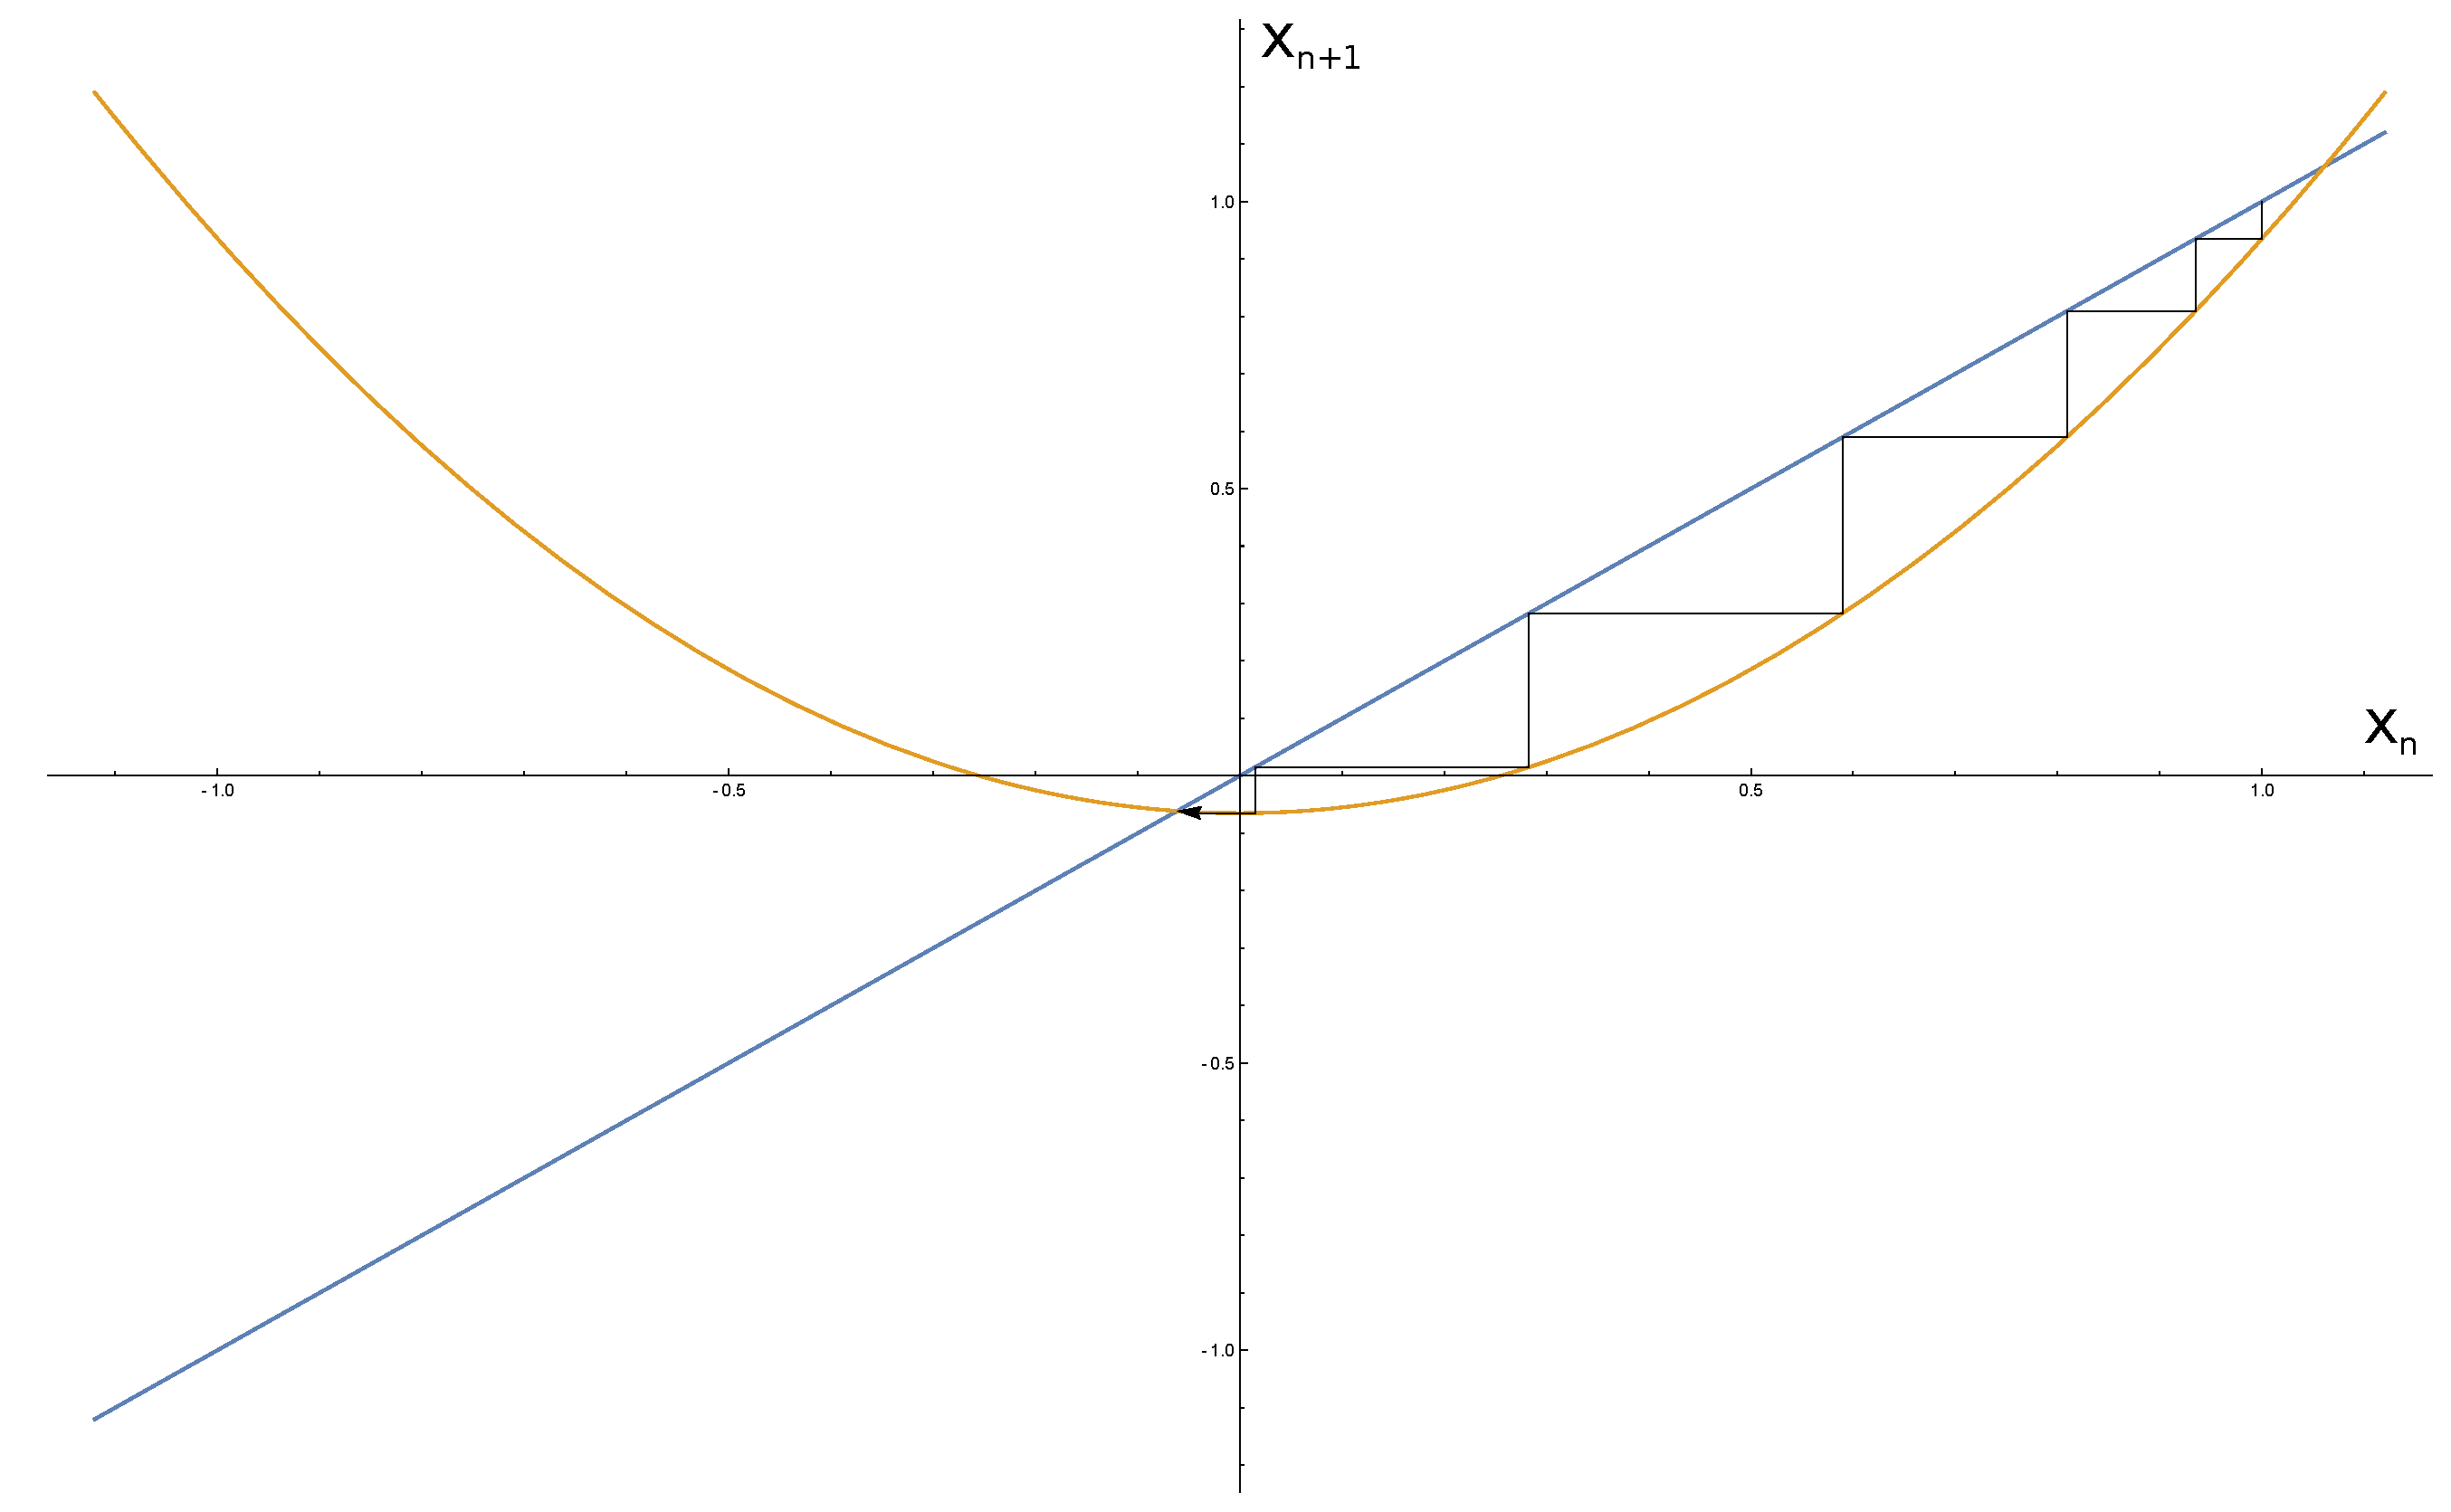
\includegraphics[width=.75\textwidth]{\imgdir/graphit.pdf}
	\caption{Graphical Iteration on $x^2 - 0.1$ with $x_0 = 1$}
	\label{graphit}
\end{figure}

A different picture that is often used for the study of a one dimensional dynamical system is an Orbit Diagram. An Orbit Diagram is a picture in parameter$\times$phase space created by sampling a range of parameter values, computing the first $n$ iterates of some seed value, and then plotting the last $m$ of those $n$ points. The images shown in Figures \ref{fig:orbits} and \ref{fig:orbits2} were made by plotting the $400^{th}$ through $500^{th}$ iterates for 20,000 uniformly sampled parameter values. The reason why these images are useful is because they roughly show how long term behaviors are changing as the chosen parameter varies: by 400 to 500 iterates most points have either escaped or fallen into some bounded pattern, thus giving an approximation of long term behavior. Typically critical points are chosen as the seed value for such a plot; again we will discuss the reasons for this choice in Chapter 3.

A final numerical technique which is useful for maps of the plane is the creation of escape pictures which quickly express the escape rates for different seed values in the plane. Typically we use two types of escape pictures: one which is in phase space and the other which is in parameter space. Phase space pictures fix all parameters and take each ``pixel'' as an initial condition in the plane to be iterated. The pixel for each point is then colored according to the relative amount of time that is takes to escape (where escape is typically determined by some iterate landing outside a ball of some predetermined radius). Similarly, a parameter space image takes each pixel as a parameter value and then iterates a critical point, recording escape in a similar manner to the phase space images. Figure \ref{fig:escape} shows two parameter space escape images and two phase space escape images for the quadratic and perturbed maps.

\begin{figure}[h]
	\centering
	\begin{subfigure}[b]{0.4\textwidth}
			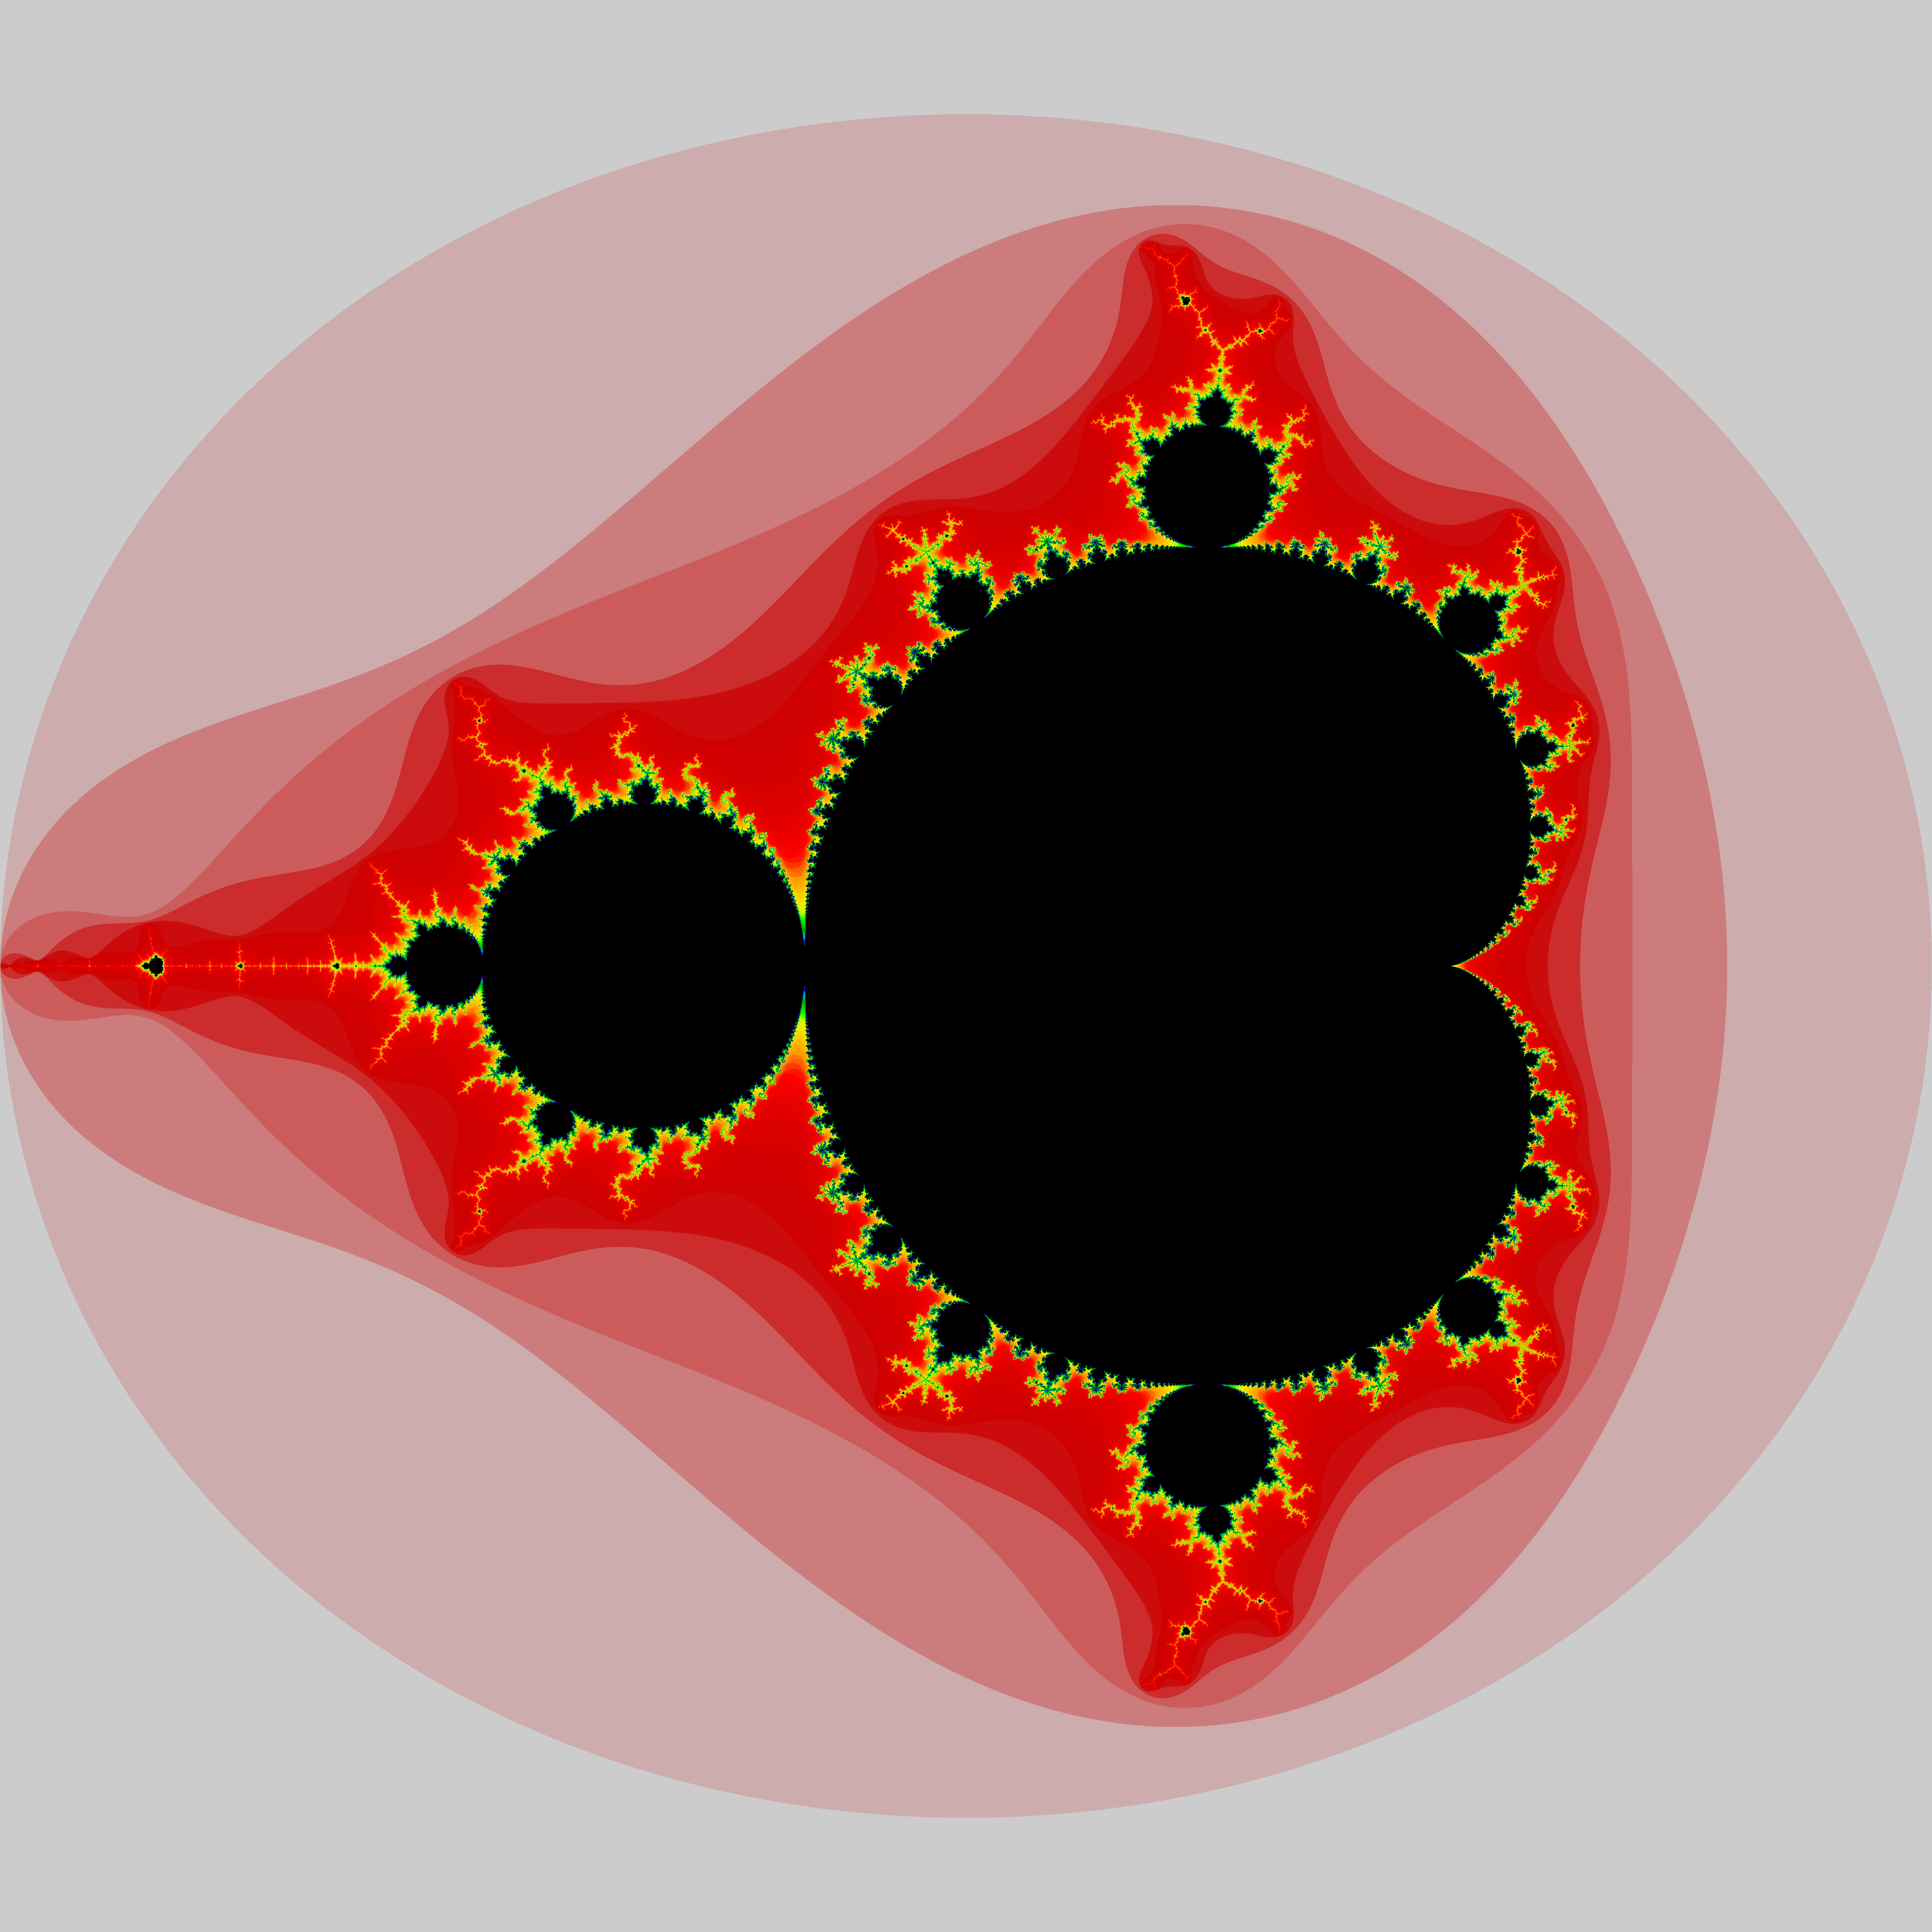
\includegraphics[width=\textwidth]{./img/b000}
			\caption{Parameter Space Escape image for $z^2 + c$ (Mandelbrot set)}
			\label{stande}%
	\end{subfigure}
	\begin{subfigure}[b]{0.4\textwidth}
			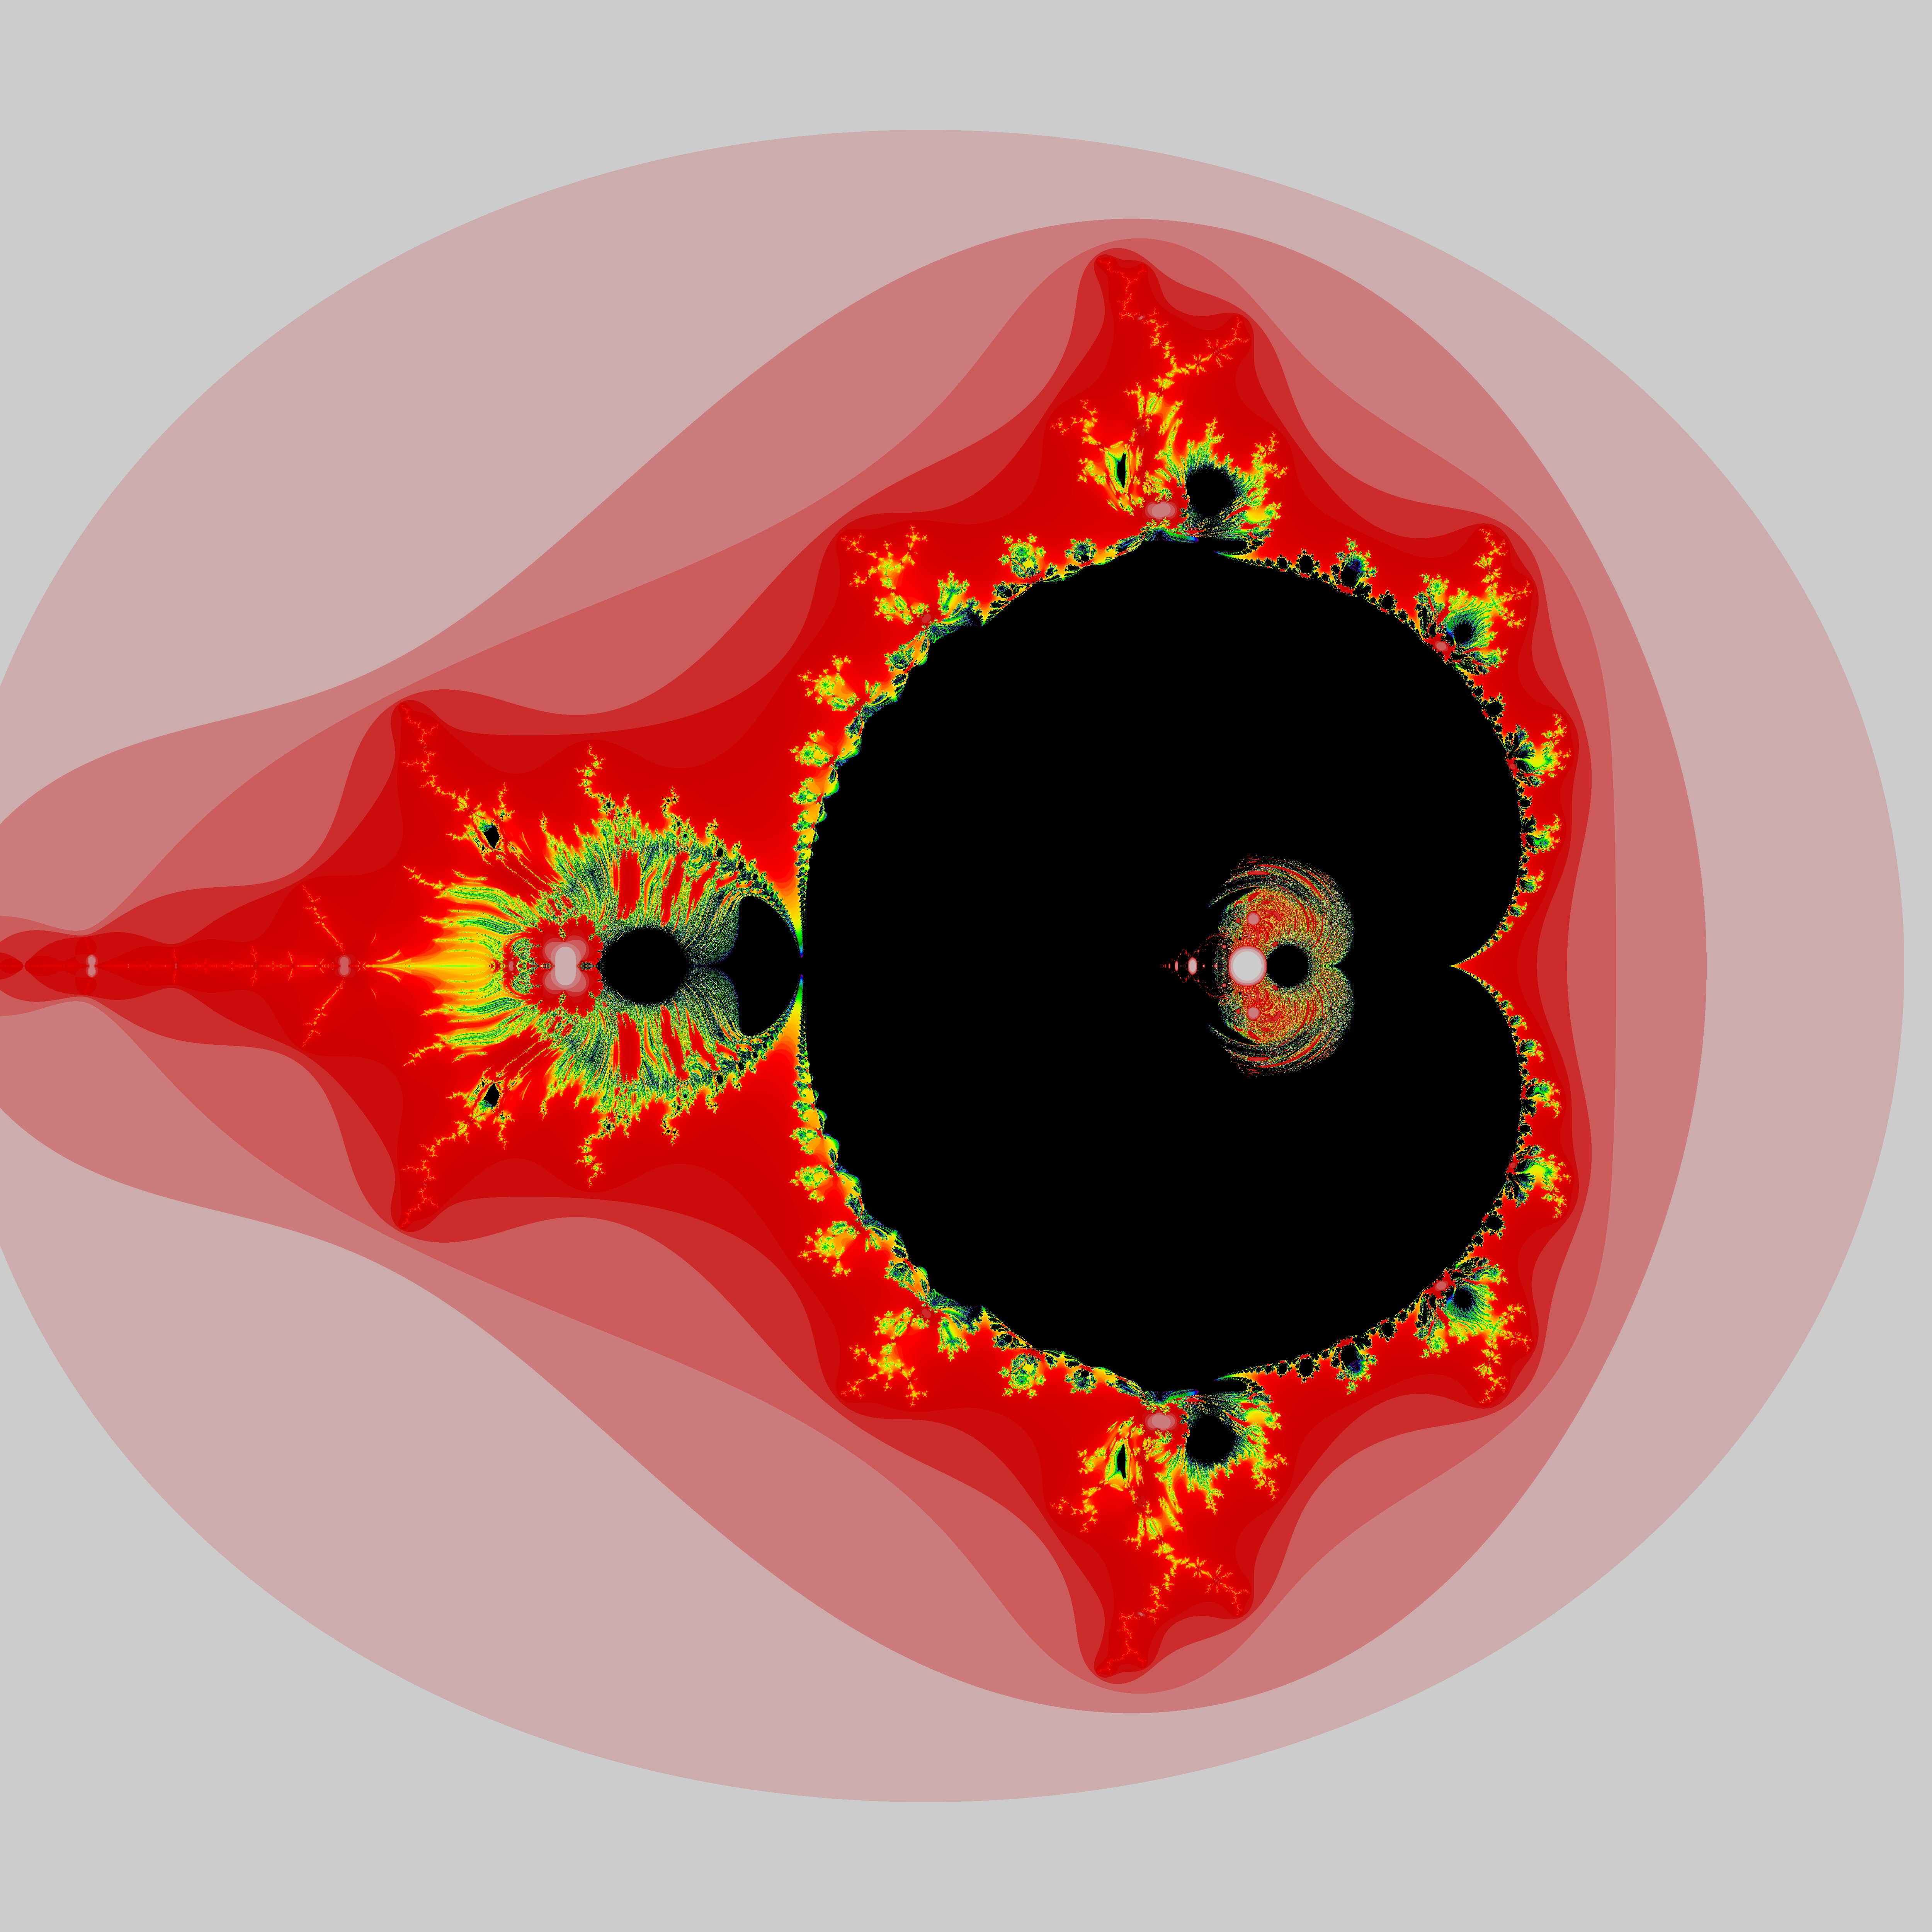
\includegraphics[width=\textwidth]{./img/b001}
			\caption{Parameter Space Escape image for $z^2 + c + \frac{.001}{\overline{z}^2}$}
			\label{perte}
	\end{subfigure}%

	\begin{subfigure}[b]{0.4\textwidth}
			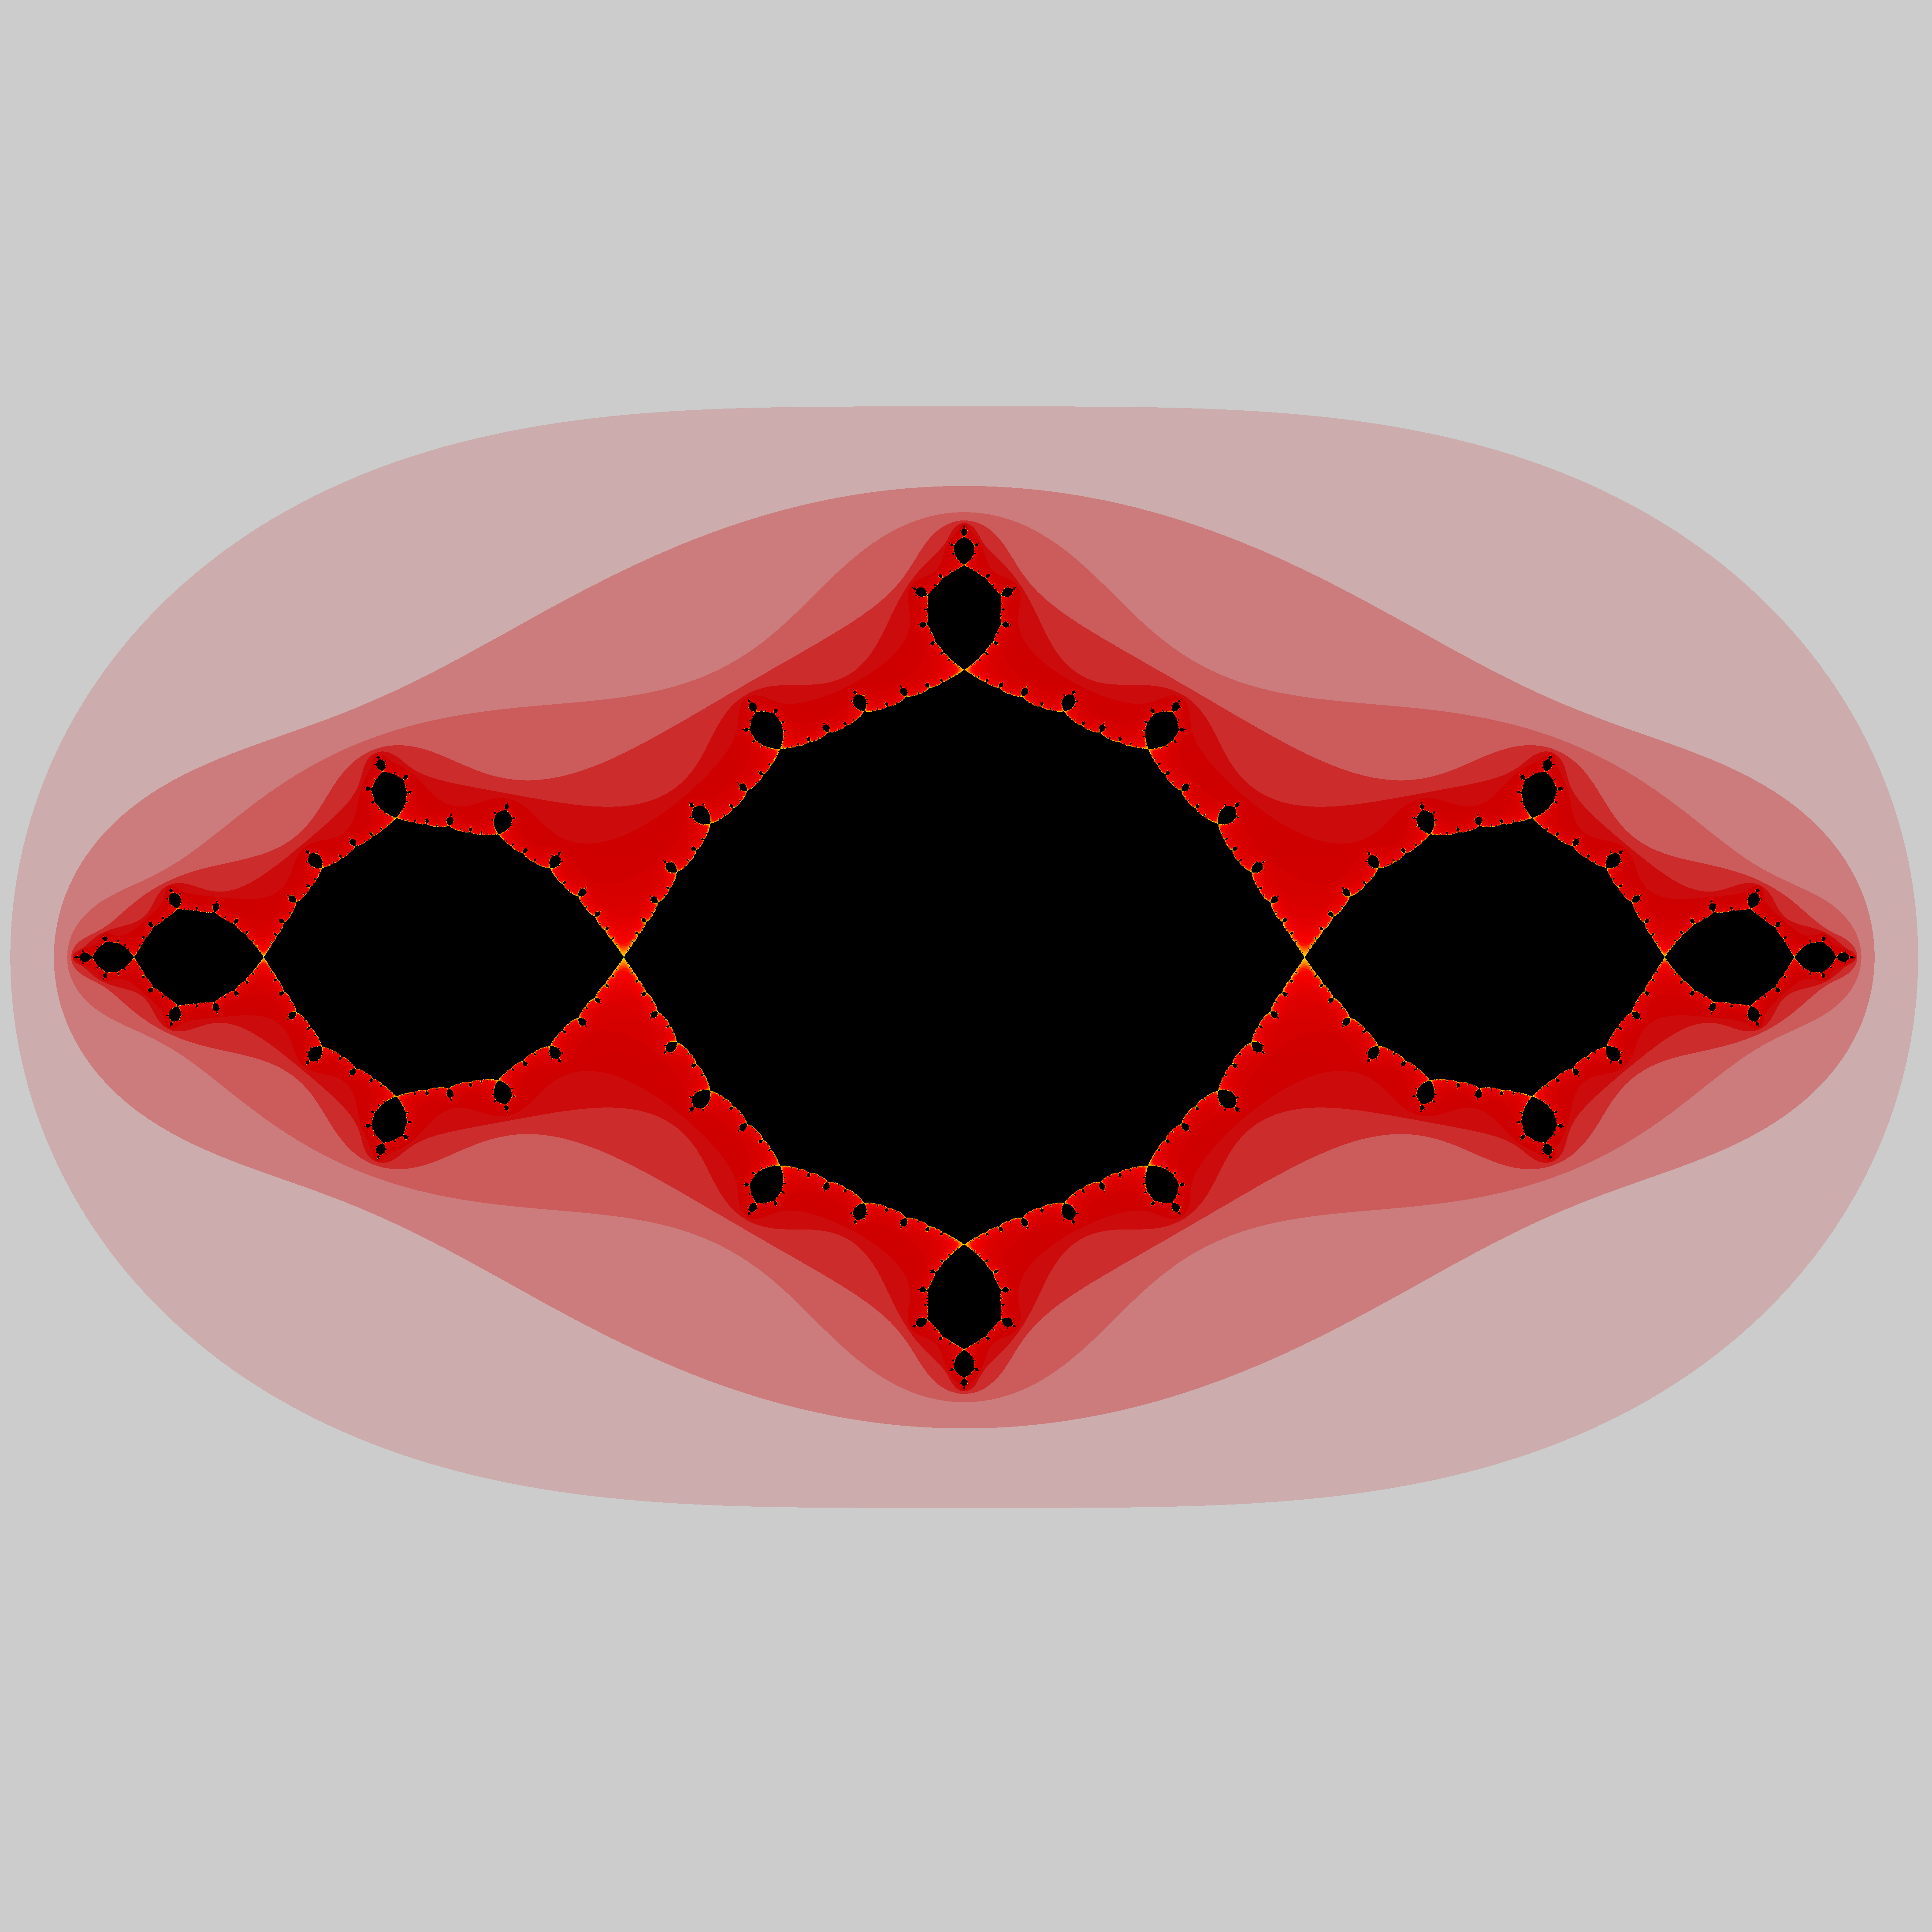
\includegraphics[width=\textwidth]{./img/phase1}
			\caption{Phase Space Escape image for $z^2 - 1$}
			\label{stande2}%
	\end{subfigure}
	\begin{subfigure}[b]{0.4\textwidth}
			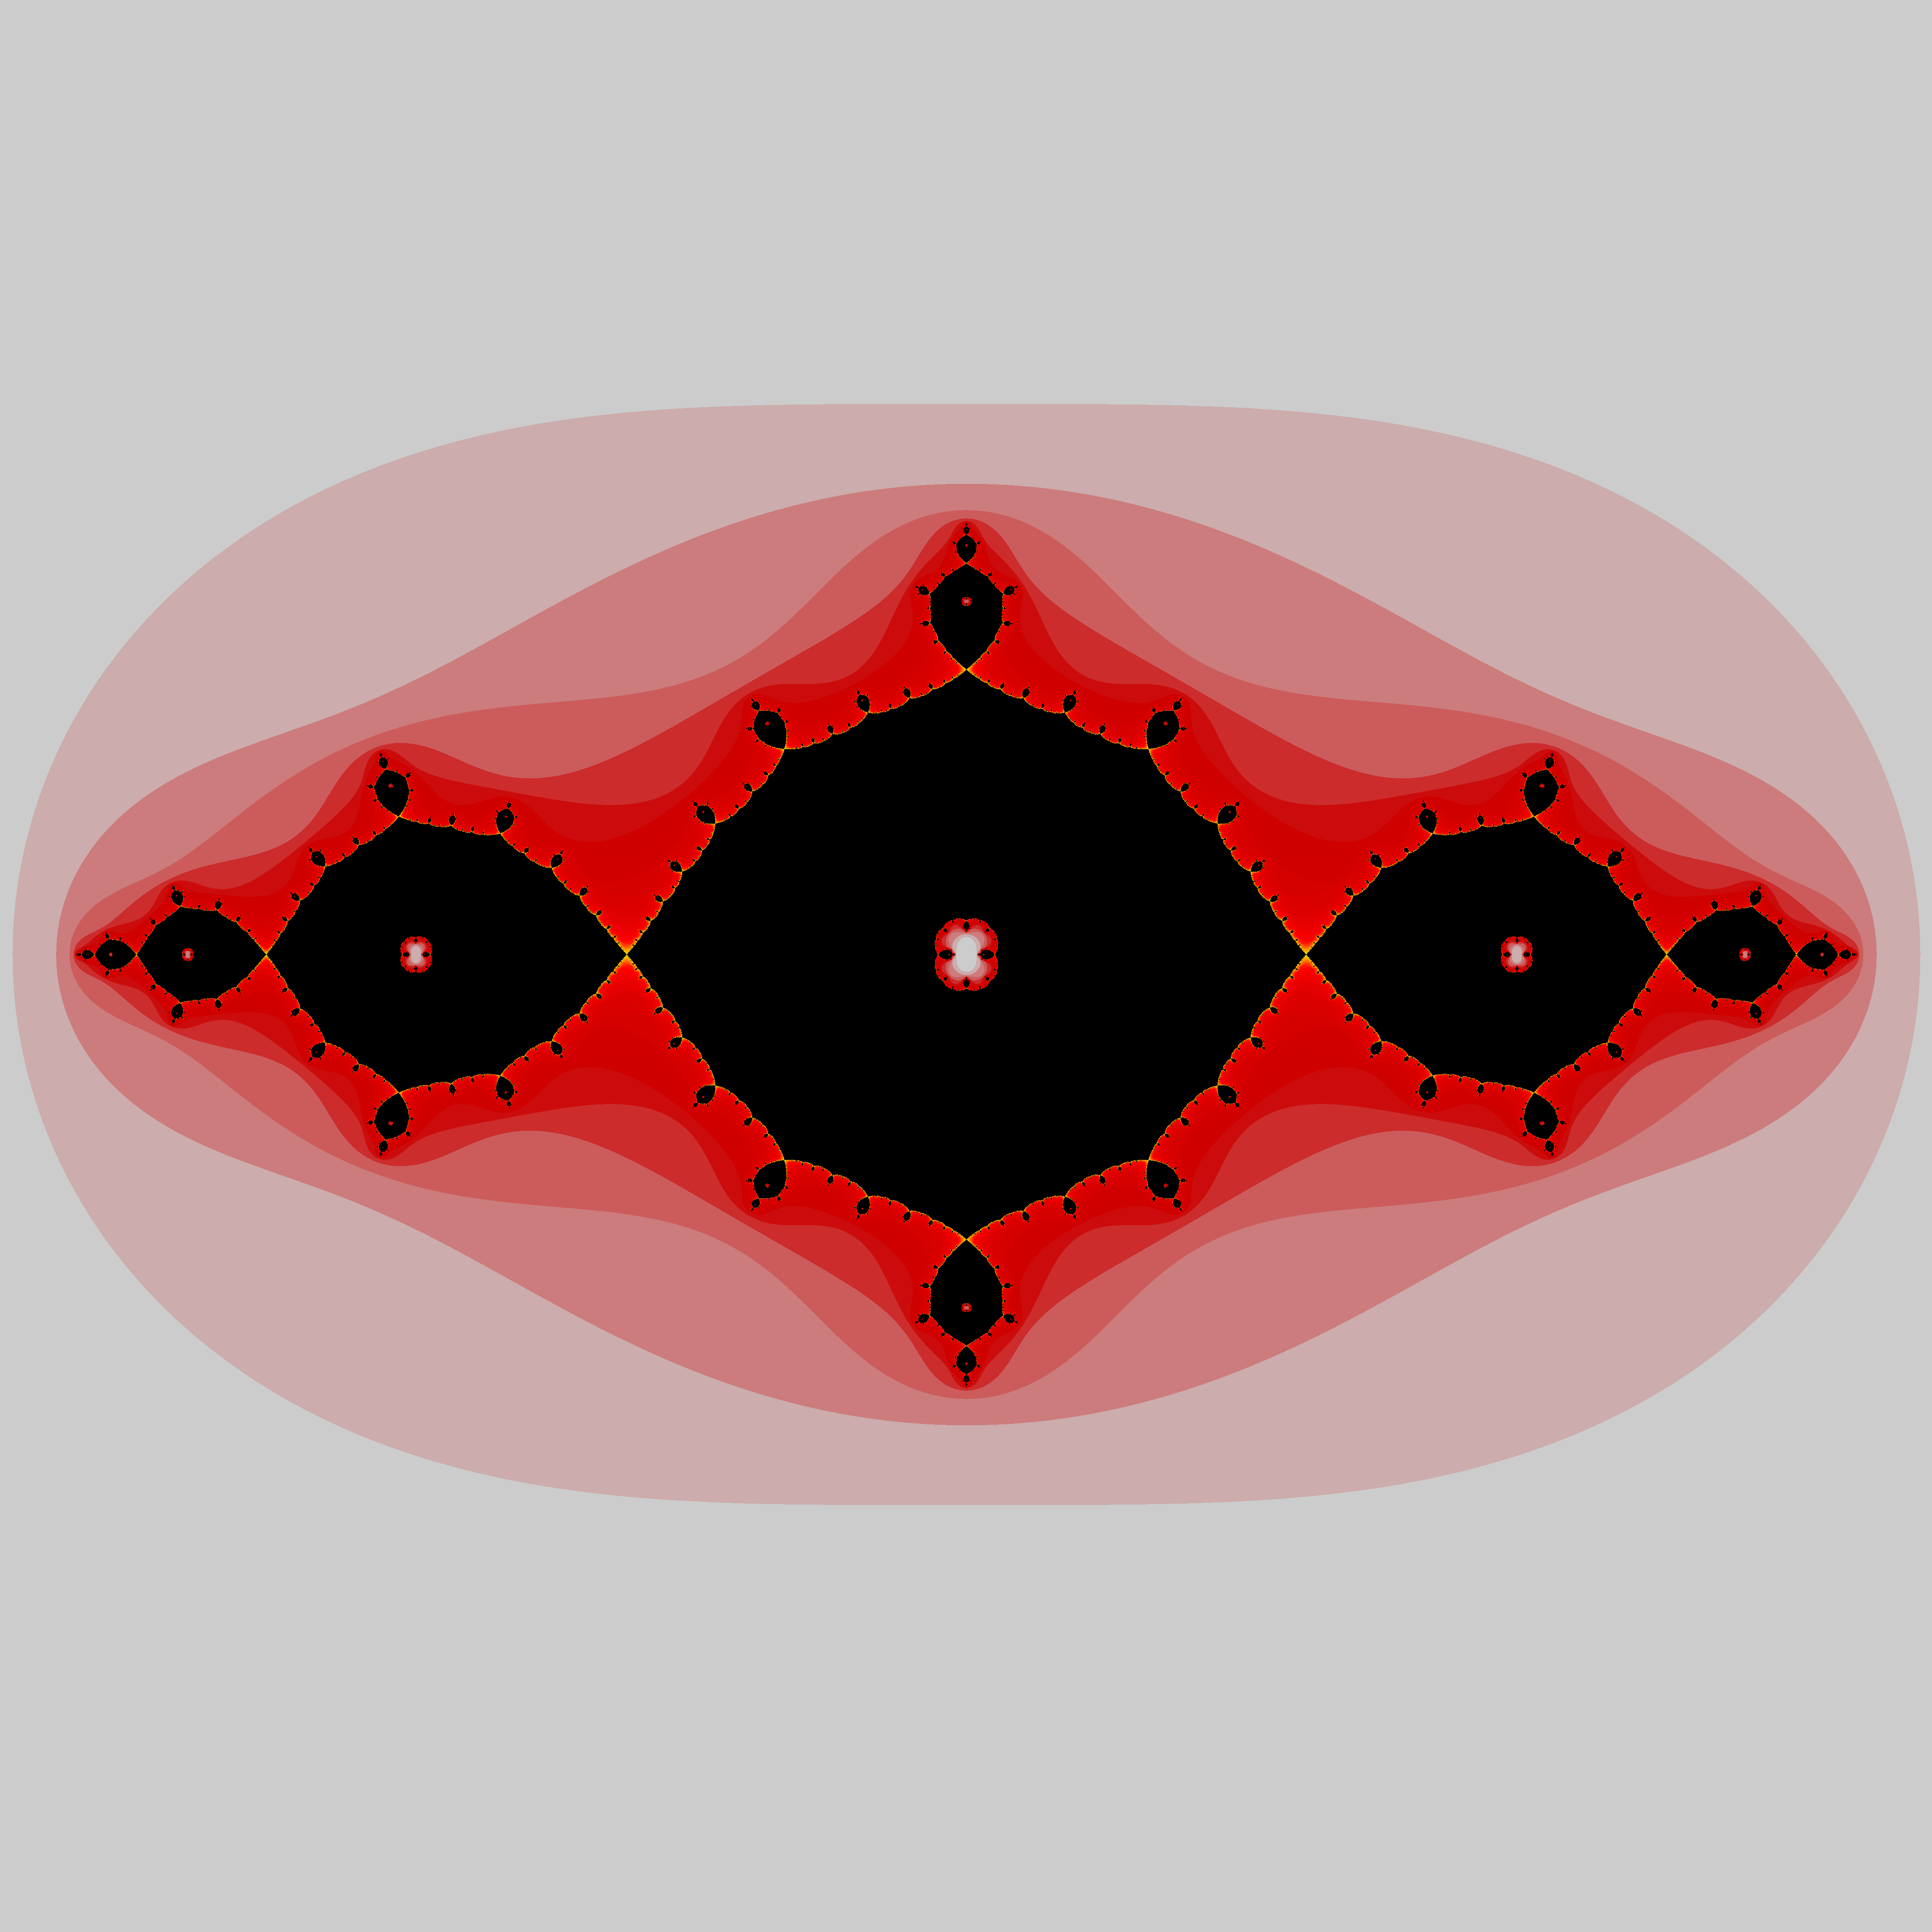
\includegraphics[width=\textwidth]{./img/phase2}
			\caption{Phase Space Escape image for $z^2 - 1 + \frac{.001}{\overline{z}^2}$}
			\label{perte2}
	\end{subfigure}%
	\caption{Escape diagrams for the quadratic and perturbed families}\label{fig:escape}
\end{figure}

\FloatBarrier
% \section{Summary of Quadratic Map Behavior}

% NEEDED?
